\newpage
\section{Comparación de la Satisfacción del Cliente en Tres Sucursales}
\subsection{Enunciado}
\textbf{Contexto:}
Una cadena de tiendas quiere comparar el nivel de satisfacción del cliente entre tres sucursales (Cochabamba, La Paz y Santa Cruz).
La satisfacción del cliente se mide en una escala de 1 a 10 (o el valor de la variable cuantitativa que identifiquen en cada sucursal,
y la empresa desea saber si existen diferencias significativas en la satisfacción entre las sucursales o la propiedad que están estudiando.

\textbf{Instrucciones:}
Obtén una muestra de puntajes de satisfacción del cliente o la variable que están analizando, para cada una de las tres sucursales.
Realiza un ANOVA de una vía para evaluar si hay diferencias significativas en el nivel de satisfacción entre las tres sucursales.

\textbf{Hipótesis:}
H0: Las medias de satisfacción del cliente son iguales en las tres sucursales.
H1: Al menos una de las medias de satisfacción del cliente es diferente entre las sucursales.

\textbf{Indicaciones:}
Usa un nivel de significancia de \(\alpha=0.05.\)

\subsection{Aplicación de la prueba en el dataset HR Employee Attrition}

\textbf{Contexto:}
Con el dataset seleccionado, lo que se quiere comparar es lo siguiente: la Satisfacción del Trabajo con 
cada departamento que exista en el dataset, en este caso podemos encontrar que existen 3 departamentos, 
Sales (Ventas), Research \& Development (Investigación y Desarrollo) y Human Resources (Recursos Humanos).
La satisfacción del trabajo se mide en una escala de 1 a 4, por lo cual para nosotros será por cada departamento.

\textbf{Y tenemos como las siguientes hipótesis:}

\begin{itemize}
    \item $H_0$: Las medias de satisfacción de trabajo son iguales en los tres departamentos.
    \item $H_1$: Al menos una de las medias de satisfacción de trabajo es diferente entre los tres departamentos.
\end{itemize}

Se tiene en cuenta también que el nivel de significancia es de \(\alpha=0.05.\)

Por lo tanto se realiza la prueba de ANOVA de una vía para evaluar si hay diferencias significativas 
en el nivel de satisfacción entre los tres departamentos.

\begin{verbatim}
import pandas as pd
import scipy.stats as stats

df = pd.read_csv('HR Employee Attrition.csv')

# Variables seleccionadas
categ_var = 'Department'  # Variable categórica
quant_var = 'JobSatisfaction'  # Variable cuantitativa

# Mostrar los elementos únicos de la variable categórica
print(f"Grupos a comparar en '{categ_var}': {df[categ_var].unique()}")
# Grupos a comparar en 'Department': ['Sales' 'Research & Development' 'Human Resources']


# Agrupar datos por la variable categórica
grupos = [df[quant_var][df[categ_var] == grupo] for grupo in df[categ_var].unique()]

# Mostrar los tamaños de los grupos
for grupo, nombre in zip(grupos, df[categ_var].unique()):
    print(f"Grupo '{nombre}' tiene {len(grupo)} observaciones.")
    # Grupo 'Sales' tiene 446 observaciones.
    # Grupo 'Research & Development' tiene 961 observaciones.
    # Grupo 'Human Resources' tiene 63 observaciones.

# Aplicando ANOVA
f_stat, p_valor = stats.f_oneway(*grupos)

print(f"\nEstadístico F: {f_stat:.4f}")
print(f"Valor p: {p_valor:.4f}")
# Estadístico F: 0.5021
# Valor p: 0.6053

# Interpretación del p-valor
alpha = 0.05
if p_valor < alpha:
    print("Rechazamos la hipótesis nula: Hay diferencias significativas entre los grupos.")
else:
    print("No rechazamos la hipótesis nula: No hay evidencia suficiente para decir que los grupos son diferentes.")

# No rechazamos la hipótesis nula: No hay evidencia suficiente para decir que los grupos son diferentes.
\end{verbatim}

Tomando en cuenta el código se compartió se hace la siguiente explicación:
\begin{itemize}
    \item Se importan las librerías necesarias.
    \item Se lee el dataset y se seleccionan las variables categórica y cuantitativa.
    \item Se muestra los grupos a comparar en la variable categórica.
    \item Se muestra el tamaño de los grupos, en nuestro caso son los departamentos.
    \item Se aplica el análisis de varianza (ANOVA) y se obtienen el estadístico F: 0.5021 y el valor p.: 0.6053 
    \item Se interpreta el resultado del p-valor.
    \item Se toma la decisión de no la hipótesis nula, porque no hay evidencia suficiente para decir que los 
    departamentos son diferentes.  
\end{itemize}

Se muestra el gráfico de boxplot para visualizar la distribución de la satisfacción del trabajo en cada departamento.

\begin{figure}[H]
    \centering
    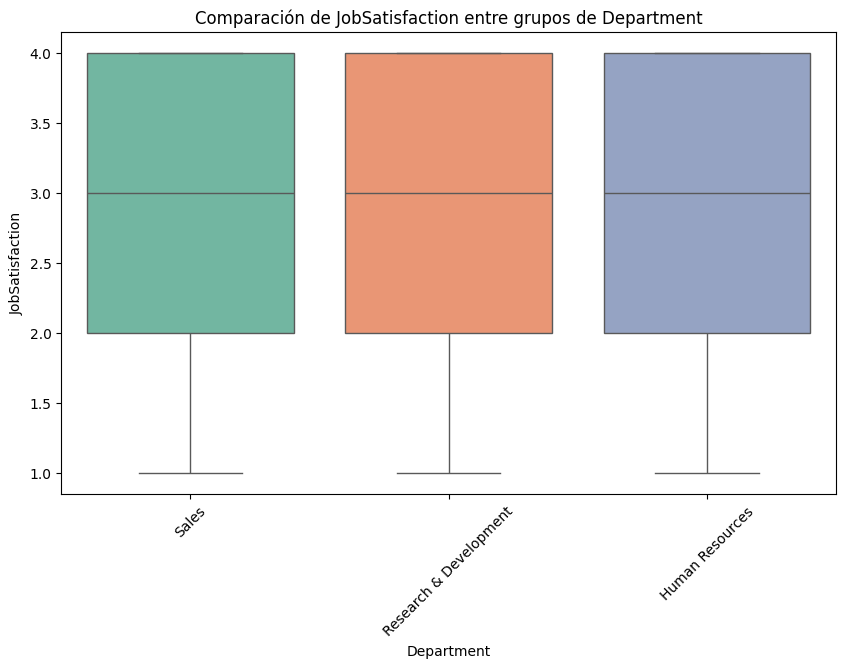
\includegraphics[width=1\textwidth]{images/boxplot-eje2.png}
    \caption{Comparación de la satisfacción del trabajo por departamento}
    \label{fig:anova}
\end{figure}


Se puede mostrar también en el siguiente gráfico mostrando lo mismo que el análisis de ANOVA. \cite{code}

\begin{figure}[H]
    \centering
    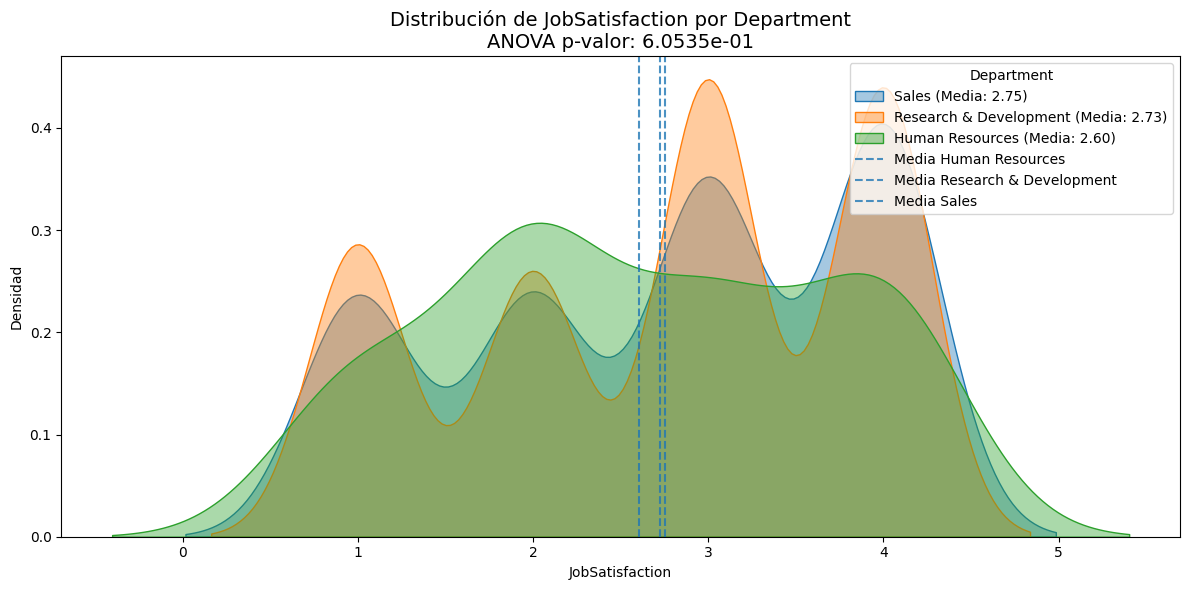
\includegraphics[width=1\textwidth]{images/sesgado-eje2.png}
    \caption{Distribución de JobSatisfaction por Department}
    \label{fig:anova-sesgado}
\end{figure}


\textbf{Conclusión:}
La hipótesis nula establece que las medias de satisfacción de trabajo son iguales en los tres departamentos. 
Dado que no se encontró evidencia estadística significativa para rechazar la hipótesis nula, podemos concluir que:

\begin{itemize}
    \item No hay diferencias significativas en la satisfacción de trabajo promedio entre los departamentos, 
    como se puede ver en ambos gráficos, especialmente en el segundo donde tienen una media muy parecida.
    \item Este resultado nos muestra que, en términos de satisfacción de trabajo, los departamentos están funcionando de manera similar.
\end{itemize}